
%(BEGIN_QUESTION)
% Copyright 2006, Tony R. Kuphaldt, released under the Creative Commons Attribution License (v 1.0)
% This means you may do almost anything with this work of mine, so long as you give me proper credit


\noindent
{\bf Wiring diagram requirements}

Perhaps the most important rule to follow when drafting a wiring diagram is {\it your diagram should be complete and detailed enough that even someone who is not a technician could understand where every wire should connect in the system!}

\begin{itemize}
\item{} {\bf Field device symbols}
\item{} Proper electrical symbols and designations used for all field devices.
\item{} {\it Optional:} Trip settings written next to each process switch.
\end{itemize}

\begin{itemize}
\item{} {\bf PLC I/O cards}
\item{} All terminals labeled, even if unused in your system.
\item{} Model number, I/O type, and PLC slot number should be shown for each and every card.
\end{itemize}

\begin{itemize}
\item{} {\bf Connection points}
\item{} All terminals properly labeled.
\item{} All terminal blocks properly labeled.
\item{} All junction (``field'') boxes shown as distinct sections of the loop diagram, and properly labeled.
\item{} All control panels shown as distinct sections of the loop diagram, and properly labeled.
\item{} All wire colors shown next to each terminal.
\item{} All terminals on devices labeled as they appear on the device (so that anyone reading the diagram will know which device terminal each wire goes to).
\end{itemize}

\begin{itemize}
\item{} {\bf Energy sources}
\item{} All power source intensities labeled (e.g. ``24 VDC,'' ``120 VAC,'' ``480 VAC 3-phase'')
\item{} All shutoff points labeled (e.g. ``Breaker \#5,'' ``Valve \#7'')
\end{itemize}

\vfil \eject

\noindent
{\bf Sample Input Wiring Diagram}

$$\includegraphics[width=15.5cm]{i01880x01.eps}$$


\vfil \eject

\noindent
{\bf Sample Output Wiring Diagram}

$$\includegraphics[width=15.5cm]{i01880x02.eps}$$


\underbar{file i01880}
%(END_QUESTION)





%(BEGIN_ANSWER)

Your loop diagram will be validated when the instructor inspects the loop with you and the rest of your team.

%(END_ANSWER)





%(BEGIN_NOTES)


%INDEX% Lab exercise, PLC I/O wiring diagram template and requirements

%(END_NOTES)


